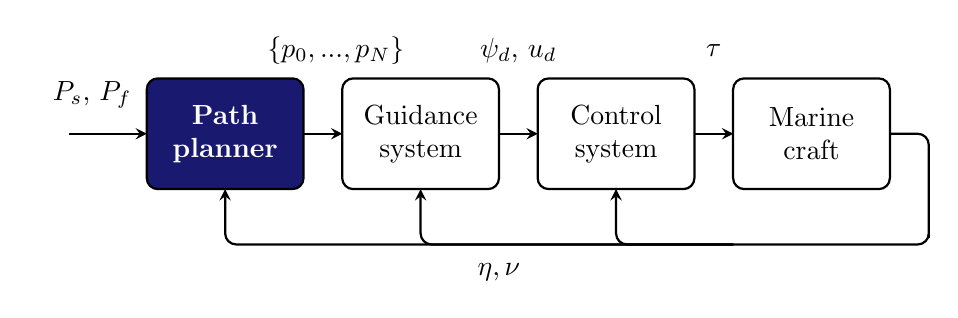
\begin{tikzpicture}[x=5.65em,y=4em]

	\tikzstyle{block} = [rectangle, draw, thick,
    		text width=5em, text centered, rounded corners, minimum height=4em]
	\tikzstyle{block_marked} = [block, fill=MidnightBlue, text=white, font=\bfseries]
	\tikzstyle{plaintext} = [draw=none,fill=none,text width=4em, text centered]
	\tikzstyle{line} = [draw, ->,>=stealth, thick, rounded corners]

    % Place nodes
    %\node [block] at (0, 0) {Mission planner};
    \node [block_marked] at (1.25, 0) {Path planner};
    \node [block] at (2.5, 0) {Guidance system};
    \node [block] at (3.75, 0) {Control system};
    \node [block] at (5, 0) {Marine craft};
    %\node [block] at (5, -2) {Navigation system};
    
    %\node [plaintext] at (-1,0) {Goal};
    \node [plaintext] at (0.4,0.35) {$P_s$, $P_f$};
    \node [plaintext] at (1.875,0.75) {$\{\boldsymbol{p}_0,...,\boldsymbol{p}_N\}$};
    \node [plaintext] at (3.125,0.75) {$\psi_d$, $u_d$};
    \node [plaintext] at (4.375,0.75) {$\tau$};
    \node [plaintext] at (3,-1.25) {$\boldsymbol{\eta}, \boldsymbol{\nu}$};
    
    
    %\path [line] (-0.75, 2) -- (0,2) |- (0, 0.5);
    %\path [line] (-0.75, 2) -- (1.25,2) |- (1.25, 0.5);
    %\path [line] (-0.75, 0) -- (-0.5,0);
    \path [line] (0.25, 0) -- (0.75,0);
    \path [line] (1.75, 0) -- (2,0);
    \path [line] (3, 0) -- (3.25,0);
    \path [line] (4.25, 0) -- (4.5,0);
    
    \path [line] (5.5, 0) -- (5.75,0) |- (5.75,-1) -- (4.5, -1) -- (3.75,-1) -- (3.75,-0.5);
    \path [line] (4.5, -1) -- (2.5,-1) -- (2.5,-0.5);
    \path [line] (4.5, -1) -- (1.25,-1) -- (1.25,-0.5);
    %\path [line] (4.5, -2) -- (0,-2) -- (0,-0.5);
    
\end{tikzpicture}